

Før den mest optimerede Huffman algoritme kan laves, er man nødt til at vide hvilke tegn der optræder oftest. Tegnene der forekommer hyppigst kommer altså helt i top i Huffman træet.

Som udgangspunkt vi at kigge på hele den danske Wikipedias indhold, da det som udgangspunkt var den største offentligt tilgængelige database for dansksprogede artikler vi kunne finde. Dette resulterede i at vi fik hentet over 340.000 danske artikler fra den frie encyklopædi. Hele denne mængde tekst blev kørt igennem et dertil indrettet program[INDSÆT EVT REFERENCE HER!!], som kunne læse samtlige tegn, tælle dem sammen og sortere efter hyppighed. Programmet er nærmere beskrevet i afsnittet ”[INDSÆT AFSNITSNAVN HER!!]”.  Med resultatet af optællingen i hånden, går det imidlertid op for os at der er en del tegn der er enten urealistisk højt eller lavt på listen. Det er fx tegn som ”=” og ”0” der ligger højt på listen, og tegn som ”:” og ”)” der ligger meget lavt på listen. Dette skyldes at der, naturligvis, ikke bliver brugt ret mange humørikoner i artiklerne. Se tabel \ref{wikiSMS2}.

\begin{table}[hba]
\begin{center}
\newcolumntype{g}{>{\columncolor{gray90}}c}
\begin{tabular}{| g | c | r || c | r |}
    \hline
    \cellcolor{ForestGreen}\color{white}{\textbf{\#}} & \multicolumn{2}{|c|}{\cellcolor{ForestGreen}\color{white}{\textbf{Wikipedia}}} & \multicolumn{2}{|c|}{\cellcolor{ForestGreen}\color{white}{\textbf{SMS}}} \\
    \hline
     1 & {[ ]} & 62.599.053 & {[ ]} & 120.208 \\ \hline
     2 & e &  62.599.053 &  e & 68.747 \\ \hline
     3 & r &  38.687.981 &  r & 35.440 \\ \hline
     4 & n &  22.736.041 &  d & 28.923 \\ \hline
     5 & t &  21.429.086 &  a & 28.244 \\ \hline
     6 & a &  18.515.100 &  t & 27.766 \\ \hline
     7 & i &  17.612.087 &  n & 27.551 \\ \hline
     8 & s &  16.237.042 &  i & 27.244 \\ \hline
     9 & l &  15.791.561 &  g & 22.990 \\ \hline
    10 & o &  14.262.580 & l & 21.244 \\ \hline
    11 & d &  14.219.812 & s & 20.787 \\ \hline
    12 & g &  10.866.430 & k & 18.928 \\ \hline
    13 & m &   8.299.169 & o & 18.118 \\ \hline
    14 & k &   7.698.281 & m & 15.358 \\ \hline
    15 & f &   6.097.333 & v & 11.819 \\ \hline
    16 & u &   5.521.282 & . & 11.556 \\ \hline
\end{tabular} 
\quad
\begin{tabular}{| g | c | r || c | r |}
    \hline
     \cellcolor{ForestGreen}\color{white}{\textbf{\#}} & \multicolumn{2}{|c|}{\cellcolor{ForestGreen}\color{white}{\textbf{Wikipedia}}} & \multicolumn{2}{|c|}{\cellcolor{ForestGreen}\color{white}{\textbf{SMS}}} \\
    \hline
    17 & v   & 5.227.432 &  u   & 9.699 \\ \hline
    18 & b   & 5.124.895 &  h   & 9.693 \\ \hline
    19 & p   & 4.901.561 &  :   & 8.396 \\ \hline
    20 & h   & 4.677.737 &  å   & 7.610 \\ \hline
    21 & .   & 4.102.220 &  f   & 7.396 \\ \hline
    22 & 1   & 3.647.961 &  j   & 7.124 \\ \hline
    23 & {=} & 3.268.579 &  p   & 6.082 \\ \hline
    24 & 0   & 2.981.855 &  {)} & 5.237 \\ \hline
    25 & c   & 2.722.686 &  b   & 5.094 \\ \hline
    26 & ,   & 2.641.834 & ?   & 4.750 \\ \hline
    27 & y   & 2.623.461 &  D   & 4.039 \\ \hline
    28 & -   & 2.492.363 &  ,   & 3.939 \\ \hline
    29 & '   & 2.314.983 & H   & 3.821 \\ \hline
    30 & 2   & 2.290.654 &  {-} & 3.749 \\ \hline
    31 & ;   & 1.966.568 & !   & 3.276 \\ \hline
    32 & 9   & 1.890.555 &  ø   & 3.122 \\ \hline
\end{tabular} 
%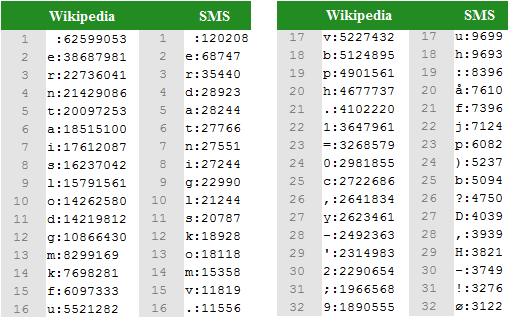
\includegraphics{Billeder/wikiVsSms.png}
\caption {Oversigt over de øverste 32 tegn.}
\label{wikiSMS2}
\end{center}
\end{table}

Det gik op for os at vi måtte analysere rigtige SMS beskeder. Snart var 13.000 SMS beskeder indsamlet og klar til analysering. Som forventet rykker tegn der indgår i humørikoner højere op på listen. Det største spring ser vi ved kolon, som rykker fra plads 53 på Wikipedia-listen til plads 19 på SMS-listen. Ydermere ser vi at ”H” går fra plads 56 på Wikipedia-listen til plads 26 på SMS-listen. Det kan forklares med at mange beskeder starter med ordet ”Hej”. Se eventuelt bilag \ref{wikiAnalyse} og \ref{SMSanalyse}. Alt dette er vi nødt til at tage hensyn til i vores implementering af Huffman algoritmen.

[SAMMENLIGNING AF ANTAL TEGN I ALT]

Eftersom vi kun har skaffet 13.000 SMS beskeder, kan vi ikke tolke resultatet entydigt. SMS’erne er indhentet fra 4 forskellige personer, hvilket groft sagt betyder at 6.500 SMS’er, altså halvdelen, er skrevet af disse 4 personer. Tallet kan endda vise sig at være endnu højere, da flere af testpersonerne kender hinanden. Dette kan skabe uligheder i resultatet hvis personerne har en speciel måde at skrive på, altså visse tegn ligger muligvis højere end de ville hvis vi havde fået skaffet beskeder fra flere end 4 personer. Det kan være tegn som ”*”, der bruges i smileys. På vores resultatliste ligger ”*” tegnet på plads nummer 47 med 1077 forekomster. 905 af disse forekomster er imidlertid kun fra én persons SMS beskeder, hvilket betyder at personen står for over 84\% af forekomsterne af tegnet - langt mere end de optimale 25\%. Det har ikke været muligt at skaffe flere SMS’er, hvilket nok er grundet at ens beskeder kan være meget personlige.

Konklusionen er at man er nødt til at tage højde for tegn der indgår i humørikoner, og nedprioritere visse tegn som ligger højt på Wikipedia-listen.
  